\documentclass[twoside, letterpaper, 12pt]{report}
\usepackage{orthodoxservicebook}
\usepackage{graphicx}
\graphicspath{ {./Images/} }
\title{The Sunday Reader's Service of the \\ \textsc{Typica}}
\date{}
\author{}

\newcommand\thrice{\instruction(3x)}
\newcommand\twelve{\instruction(12x)}
\newcommand\forty{\instruction(40x)}

\newcommand\prostration{\emph{(prostration)}}

\newcommand\lhmThree{Lord, have mercy.\thrice}
\newcommand\lhmTwelve{Lord, have mercy.\twelve}
\newcommand\lhmForty{Lord, have mercy.\forty}

\newcommand\throughtheprayers{Through the prayers of our holy fathers,
  Lord Jesus Christ our God,
  have mercy on us, and save us}
\newcommand\gne{Glory to the Father and to the Son and to the Holy Spirit,
  both now and ever, and unto ages of ages.  Amen.}
\newcommand\glory{Glory to the Father and to the Son and to the Holy Spirit,}
\newcommand\nowandever{Both now and ever and unto ages of ages.  Amen.}

\begin{document}
\maketitle
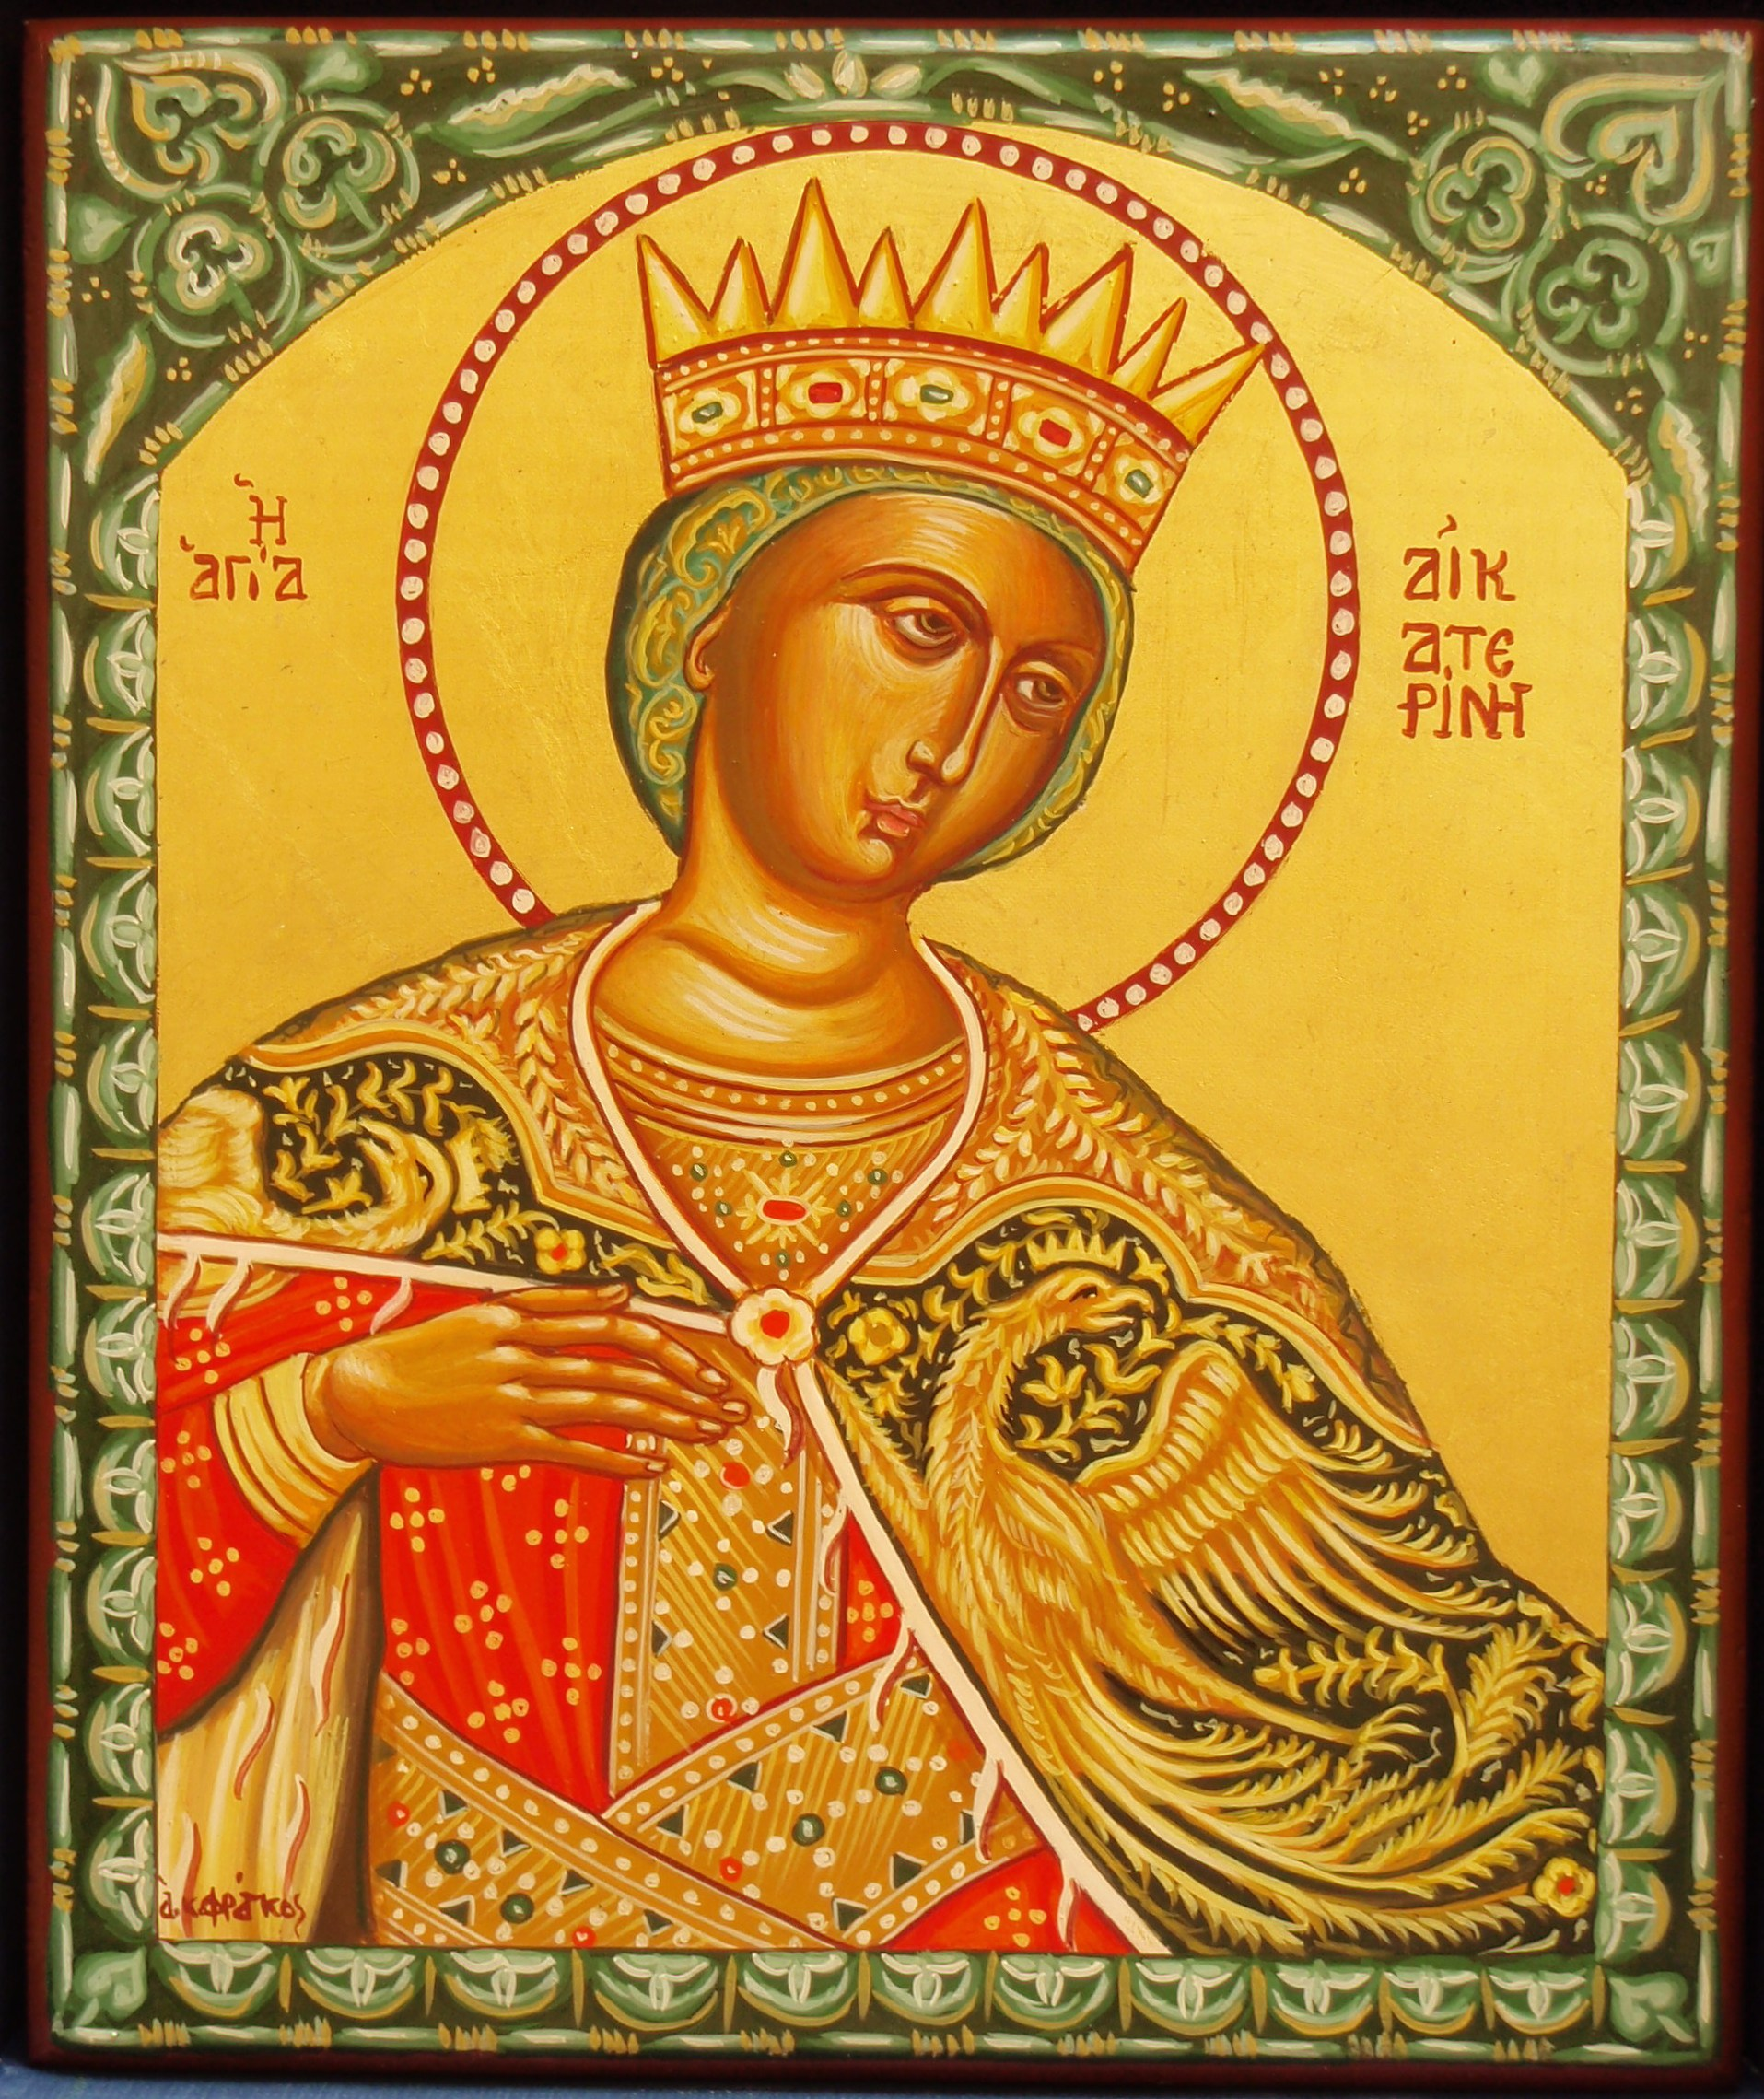
\includegraphics[width=\textwidth]{Katherine1.jpg}
\cleardoublepage

\chapter*{The Sunday Reader's Service of Typica}
\readerline{Through the prayers of our holy fathers, Lord Jesus Christ our God,
  have mercy on us, and save us}
\lilypondfile{./Common/amen.ly}
\readerline{Lord have mercy. \instruction{12x}}


\centeredsection{The First Antiphon}
\instruction{This may be replaced for certain feast days.}
\lilypondfile{./Common/bless_the_lord_greek.ly}
\readerline{Lord have mercy. \instruction{3x}}


\centeredsection{The Second Antiphon}
\instruction{This may be replaced for certain feast days.}
\lilypondfile{./Common/praise_the_lord_greek.ly}
\readerline{Lord have mercy. \instruction{3x}}


\centeredsection{The Third Antiphon}
\instruction{This may be replaced for certain feast days.}
\lilypondfile{./Common/beatitudes.ly}

\centeredsection{The Entrance Hymn}
\readerline{ Let us attend!}
\lilypondfile{./Common/entrance.ly}


\centeredsection{Troparia}
\instruction{This is modified on Great Feasts.}

\emph{The Sunday Tropar of the Resurection.}

\readerline{Glory to the Father and to the Son and to the Holy Spirit,}

\emph{The appointed Tropar of the day.}

\readerline{Now and ever and unto ages of ages.  Amen.}


\centeredsection{The Tropar of Saint Katherine}
\lilypondfile{./Common/kontak_katherine_obikhod.ly}
\readerline{Through the prayers of our holy fathers, Lord Jesus Christ our God,
  have mercy on us, and save us.}
\lilypondfile{./Common/amen.ly}


\centeredsection{The Trisagion Hymn}
\lilypondfile{./Common/trisagion_byzantine_a.ly}
\readerline{With Strength!}
\lilypondfile{./Common/trisagion_byzantine_b.ly}


\centeredsection{The Prokeimenon}
\paragraph{Reader 1}{Let us attend!}

\instruction{The second reader should be standing in front of the royal doors facing the altar}
\paragraph{Reader 2} The Prokeimenon!

\instruction{The reader then intones the prokeimenon while facing the altar}


\centeredsection{The Epistle}
\paragraph{Reader 1} Wisdom!

\instruction{The second reader continues facing the altar}
\paragraph{Reader 2} The reading from the Epistle of the holy Apostle Paul to the
  \underline{\hspace{1in}}
  
  (or from the Acts of the Holy Apostles.)
  
  (or from the Holy Epistle of Saint \underline{\hspace{1cm}}.)

\paragraph{Reader 1} Let us attend.

\instruction{The Reader turns and faces the people, and then chants the appointed Epistle,
  or Epistles for the day.}

\lilypondfile{./Common/alleluia.ly}


\centeredsection{The Gospel}
\readerline{Let us attend, the reading from the Holy Gospel according to Saint
  \underline{\hspace{1in}}.}
\lilypondfile{./Common/glory_to_thee.ly}

\readerline{\instruction{Gospel reading for the day}}
\lilypondfile{./Common/glory_to_thee.ly}

\begin{reader}
\item Lord, have mercy. \instruction{3x - (Said in place of the litany of the catechumens)}
\item Lord, have mercy. \instruction{3x - (Said in place of the first litany of the faithful)}
\item Lord, have mercy. \instruction{3x - (Said in place of the second litany of the faithful)}
\end{reader}


\centeredsection{Prayer to the Lord of Hosts}
\newcommand\metania{\emph{(metania)}}
Remember us, O Lord, when thou comest in thy kingdom.\metania

Remember us, O Master, when thou comest in thy kingdom.\metania

Remember us, O Holy One, when thou comest in thy kingdom.\metania

The heavenly choir singeth thy praises, saying: Holy, holy, holy, Lord of Sabaoth; heaven and earth are full of Thy glory.

Come unto him, and be enlightened, and your faces shall not be ashamed.

The heavenly choir singeth thy praises, saying: Holy, holy, holy, Lord of Sabaoth; heaven and earth are full of Thy glory.

\emph{Glory to the Father and to the Son and to the Holy Spirit,}

The choir of the holy angels and archangels, with all the powers of heaven, singeth thy praises, saying: Holy, holy, holy, Lord of Sabaoth; heaven and earth are full of Thy glory.

\emph{both now and ever and unto ages of ages.  Amen.}


\centeredsection{The Creed}
\instruction{Recited together as a congregation}

I believe in one God, the Father Almighty, Maker of heaven and earth,
and of all things visible and invisible.
And in one Lord Jesus Christ, the Son of God, the Only-begotten,
Begotten of the Father before all worlds, Light of Light, Very God of Very God,
Begotten, not made; of one essence with the Father, by Whom all things were made:
Who for us men and for our salvation came down from heaven,
and was incarnate of the Holy Spirit and the Virgin Mary, and became man.
And was crucified also for us under Pontius Pilate, and suffered and was buried.
And on the third day He rose again, according to the Scriptures; and ascended into
heaven, and sitteth at the right hand of the Father.
And He shall come again with glory to judge the living and the dead,
Whose Kingdom shall have no end.
And I believe in the Holy Spirit, the Lord, and Giver of Life,
Who proceeds from the Father,
Who with the Father and the Son together is worshiped and glorified,
Who spake by the Prophets.
And I believe in One Holy Catholic and Apostolic Church.
I acknowledge one Baptism for the remission of sins.
I look for the Resurrection of the dead, and the Life of the world to come.
Amen.


\centeredsection{Prayer of Forgiveness}
\readerline{Forgive, remit, pardon, O God, our sins,
  both voluntary and involuntary, in deed and in word, in knowledge or in ignorance,
  committed by night or by day, in mind and in thought.
  Forgive us them all, for thou art good and lovest mankind.
}


\centeredsection{The Lord’s Prayer}
\instruction{Recited together as a congregation}

Our Father, who art in heaven, hallowed be thy name; thy kingdom come;
thy will be done on earth, as it is in heaven. Give us this day our daily bread.
And forgive us our trespasses, as we forgive those who trespass against us.
And lead us not into temptation,but deliver us from evil.

\readerline{Through the prayers of our holy fathers, Lord Jesus Christ our God, have mercy on us.}
\lilypondfile{./Common/amen.ly}


\centeredsection{Kontakia}
\instruction{This is modified on Great Feasts.}

\centeredsubsection{Kontakion of Saint Katherine}
\lilypondfile{./Common/kontak_katherine_obikhod.ly}

\emph{The appointed Kontakion of the day.}

\readerline{\glory}

\emph{The Sunday Kontakion of the Resurrection.}

\readerline{\nowandever}

\centeredsubsection{Theotokion for Ordinary Sundays}
\instruction{This is often replaced with a Theotokion specific to the day.}

\lilypondfile{./Common/steadfast_protectress.ly}

\readerline{\lhmForty}

\lilypondfile{./Common/blessed_be_the_name_flat.ly}

\readerline{\gne}

\begin{maybetwocolumns}
\centeredsection{Psalm 33}
\input{./Psalms/Psalm033-unknowntrans.txt}

\centeredsection{Psalm 144}
\input{./Psalms/Psalm144-unknowntrans.txt}
\end{maybetwocolumns}

\readerline{\gne}


\centeredsection{The Theotokion}
\lilypondfile{./Common/truly_meet_obikhod.ly}


\centeredsection{}{The Dismissal}

\lilypondfile{./Common/dismissal_obikhod.ly}

\readerline{\throughtheprayers}

\lilypondfile{./Common/amen.ly}

\end{document}

